\section{Formgedächtnislegierungen}

\begin{frame}[t]\frametitle{Gliederung: Formgedächtnislegierungen}
\tableofcontents[
currentsection,
subsectionstyle=show/show/hide
]
\end{frame}

\subsection{Effekte}
\label{fgl:effekte}
\begin{frame}[c]\frametitle{Effekte}
	Verschiedene Effekte von Formgedächtnislegierungen:
	\begin{itemize}
		\item{Einwegeffekt}
		\item{Zweiwegeffekt}
		\item{Pseudoelastizität}
	\end{itemize}
\end{frame}

\subsection{Zweiwegeffekt}
\label{fgl:zweiwegeffekt}
\begin{frame}[t]\frametitle{Zweiwegeffekt}
	\centering
	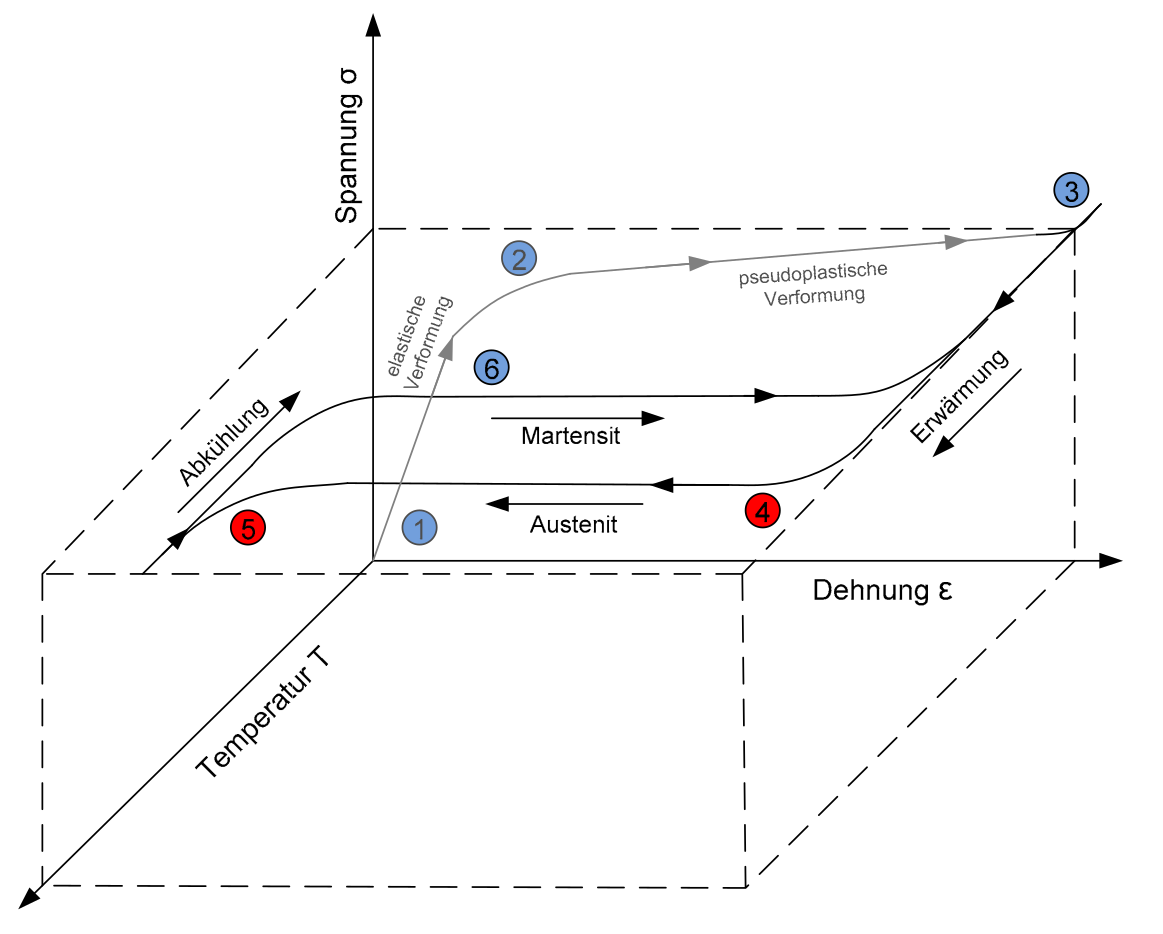
\includegraphics[height=0.5\textwidth]{medien/Verhalten_beim_Zweiwegeffekt.png}
	\\
	\tiny{Quelle: Sven Langbein \& Alexander Czechowicz. Konstruktionspraxis
	Formgedächtnistechnik. Potentiale - Auslegung - Beispiele (Seite: 7).}
\end{frame}

\begin{frame}[c]\frametitle{Zweiwegeffekt}
	\centering
	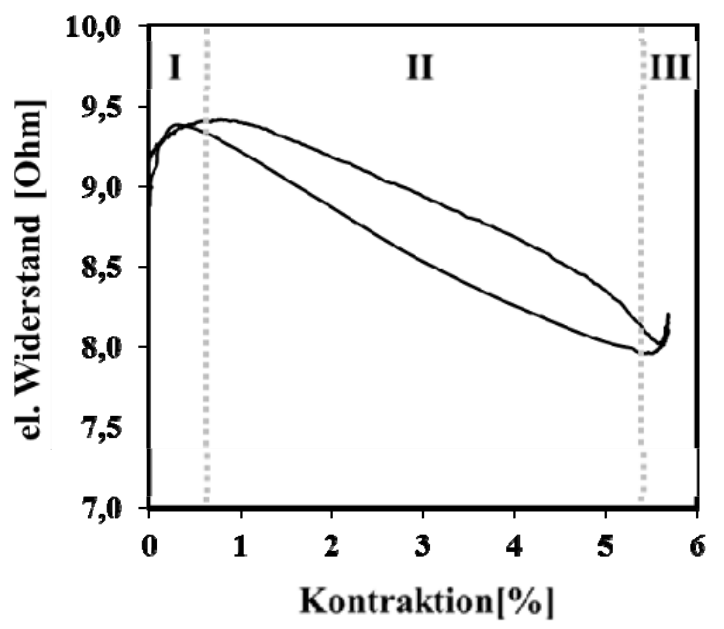
\includegraphics[height=0.5\textwidth]{medien/widerstand_zu_kontraktion.png}
	\\
	\tiny{Quelle: Sven Langbein \& Alexander Czechowicz. Konstruktionspraxis
	Formgedächtnistechnik. Potentiale - Auslegung - Beispiele (Seite: 110).}
\end{frame}

\subsection{Pseudoelastizität}
\label{fgl:pseudoelastizität}
\begin{frame}[c]\frametitle{Pseudoelastizität}
	Die Umwandlungstemperatur liegt unter der Arbeitstemperatur
	(Umgebugstemperatur), im Normalfall unter 0°C.\\
	\centering
	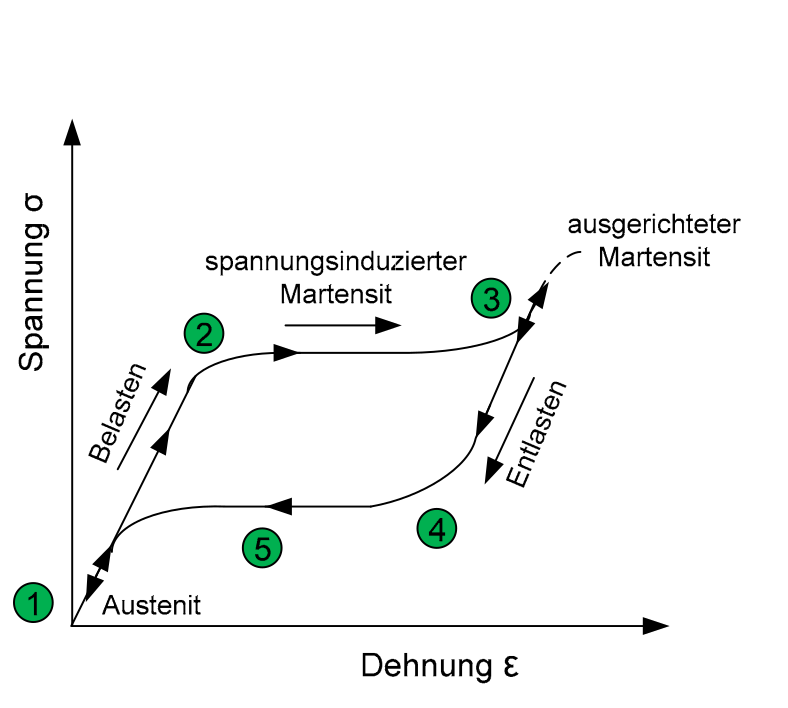
\includegraphics[height=0.5\textwidth]{medien/Verhalten_beim_pseudoelastischen_Effekt.png}
	\\
	\tiny{Quelle: Sven Langbein \& Alexander Czechowicz. Konstruktionspraxis
	Formgedächtnistechnik. Potentiale - Auslegung - Beispiele (Seite: 8).}
\end{frame}
